
\chapter*{Forord} \fxnote{Skriv det}

Kilder er refereret som en numerisk reference indrammet af firkantede parenteser, f.eks. [8]. Listen over kilder der refereres til, er samlet under afsnittet \textit{Litteraturliste}, hvor \textit{forfatter}, \textit{titel}, \textit{årstal}, og evt. \textit{link} er angivet. Refereres der til en bestemt side, anføres det ved [8, p.32]. Referencer internet i projektrapporten er anvist som \textit{Type af reference} + \textit{afsnit.nummer}, f.eks. \textit{figur 8.32}. Henvisninger til projektdokumentationen er gøres ved  angivelsen \textit{ses i dokumentationen, afsnit...}, samt angivelse af afsnittets navn.


{\let\clearpage\relax \chapter{Indledning}}
Til rumfart anvendes flere forskellige mekanismer, til frigørelse af udvendige, bevægelige dele på satellitten. Det indebærer bl.a. solpaneler, antenner, varmeskjold og mange andre. Disse mekanismer har indtil nu typisk haft brug for hver deres unikke aktiveringskredsløb. Ved udvikling af et universelt aktiveringskredsløb, kan det derfor opnås en effektivisering af pladsforbruget for disse aktiveringskredsløb. Derudover vil det også skabe et mere overskueligt system, fra forsyningskilde til udgangsbelastning. 

Fordi aktiveringskredsløbet skal bruges til rumfart, hvor afledning af varme er begrænset, er effektiviteten af effektoverførelsen fra kilde til belastning essentiel. Denne effektivitet skal optimeres for opnåelse af minimal afkølingstid, og dermed også spildtid, for effektivisering af udfoldelse af de udvendige mekanismer\cite{projekt-oplag}. 

Målet for dette bachelorprojekt er at udvikle en DC/DC converter, der kan programmeres til to forskellige foruddefinerede udgangsbelastninger. Som et fremadrettet mål, ønskes det at udgangen skal kunne programmeres til enhver ønsket belastning, indenfor en vis grænse. 

Hele aktiveringskredsløbet består af fire overordnede funktionaliteter. Terma tidligere udviklet variationer af fulde aktiveringskredsløb. Derfor er de omkringliggende kredsløb allerede udviklet, og det vil kun være aktuator modulet der vil være en del af dette bachelorprojekt.
\begin{itemize}
	\item Armeringskredsløb, der fungerer som en hovedafbryder
	\item Aktuator modul
	\item Aktuator-vælger, der består af et switch array til aktivering af aktuatoren
	\item CM-bus interface, som er et digitalt og analogt kommando interface
\end{itemize}

En oversigt over det samlede system er givet på figur~\ref{fig:system_overblik}. Dette viser de fire førnævnte blokke - armeringskredsløb, aktuator modul(converter), aktuator-vælger og CM-bus interface. Armeringskredsløbet fungerer, som en sikkerhedsanordning i det samlede kredsløb, ved først at forsyne aktuator modulet når kredsløbet er blevet armeret. Det skal forhindre fejlaktiveringer, da der vil ske materiel skade ved aktiveringer i miljø med for lidt plads. 

Aktuator modulet er converteren der ønskes designet. Den skal sætte en firkantet I/V karakteristik for aktiveringskredsløbet, der er unik for hver load type. Til dette er der to analoge signaler tilrådighed, der skal bruges som referenceværdier. Derudover er der et digitalt signal til aktivering af aktiveringskredsløbet. Det vil fungere som det endelige aktiveringssignal, der slutter den sidste kontakt til forsyningen. 

Aktuator-vælgeren består af et switch-array. Det slutter forbindelsen til den valgte load. Loaden vil blive valgt ud fra en række digitale signaler, der aktiverer kontakten til den ønskede load.

CM-bus interface'et består af et kommunikationsinterface for analoge og digitale signaler. Det bruges til kommunikation mellem et kontrolcenter og fartøjets elektriske moduler. Derudover fungerer det også som indgangskilde til aktiveringsmodulet. 

Diagrammet viser projektets to primære load typer - \textit{Pyro load} og \textit{Thermal Knife load}. Selvom det fremadrettede mål er udvikling af en converter der kan programmeres til enhver ønsket udgangsbelastning, vil der i dette projekt kun blive designet efter de førnævnte load typer.

\begin{figure}[H]
	\center
	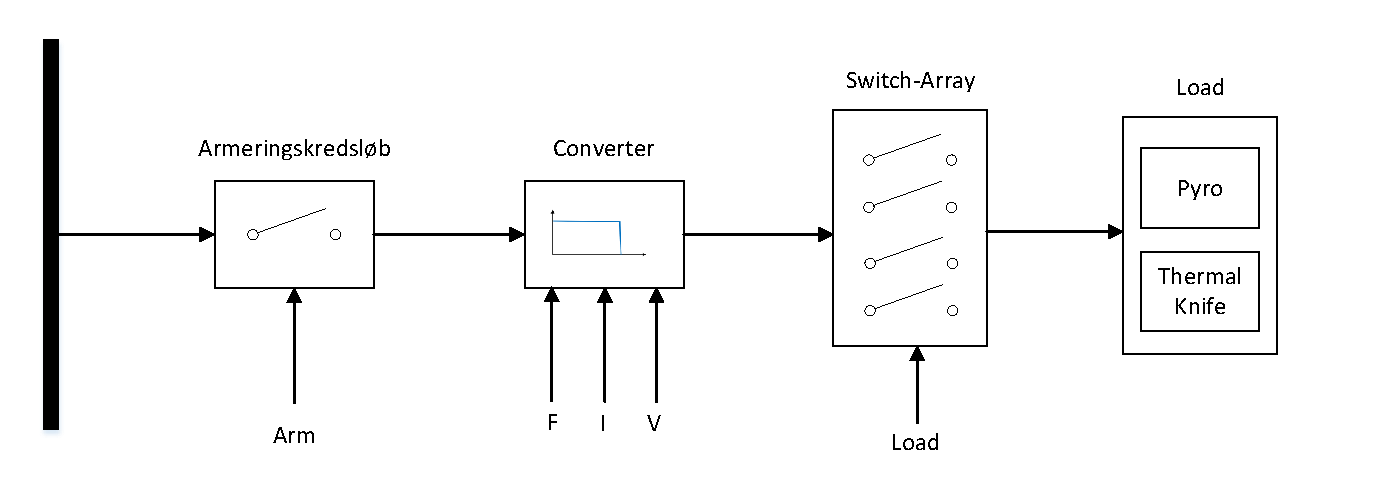
\includegraphics[max width=0.7\linewidth]{/tex/Indledning/billeder/system_overblik.pdf}
	\caption{Diagram over det samlede system}
	\label{fig:system_overblik}
\end{figure}

Projektet er udarbejdet som en iterativ udviklingsproces, hvor der hele tiden vurderes på funktionaliteten af det udviklede, og nødvendigheden for optimering. I projektet er der gennemført tre iterationer, men flere er planlagt for fremtidig videreudvikling. 


%%%%%%% Input af opgaveformuleirngen %%%%%%% 


\chapter{Opgaveformulering}
I projektet skal der udvikles en DC/DC converter, som del af et universelt aktiveringskredsløb. Converteren skal kunne operere kontinuerligt i vakuum uden overophedning. Det skal være muligt, at programmere converterens udgangsbelastning med to analoge signaler, som skal være en angivelse af henholdsvis udgangsspænding og -strøm. Converteren skal kunne holde udgangen stabil indenfor et foruddefineret interval for indgangsspændingen. Der skal implementeres en overstrøms- og overspændings-beskyttelse, der sikre beskyttelse af converteren ved kortslutning af udgangen. 

\noindent Følgende punkter skal indgå i produktet:
\begin{itemize}
	\item Holde stabil udgangsspænding, ved ændring af indspænding
	\item Præcis regulering af udgangen, efter både udgangsspænding og -strøm
	\item Programmering af udgangsbelastningen, ved to analoge spændinger
	\item Stabil regulering af udgangen, ved både laveste og højeste indgangsspænding
	\item Termisk design de er funktionsdygtigt i vakuum 
\end{itemize}

\clearpage

\section{Ordliste}
I nedenstående tabel ses en ordliste, der forklarer begreber og forkortelser, som bliver brugt i dokumentationen og rapporten.
\begin{table}[H] 			
	\centering
	\begin{tabularx}{\textwidth}{|X|l|} 
		\hline
		\textbf{Begreber} & \textbf{Forklaring} \\ \hline
		3f3 & Kernemateriale for transformator \\ \hline
		BDD & Block Definition Diagram \\ \hline
		B-felt & Magnetisk fluxtæthed \\ \hline
		CCM & Continious conduction mode \\ \hline
		DCM & Discontinoius conduction mode \\ \hline
		EEE komponenter & Komponenter der er testet og verificeret til brug i rummet \\ \hline
		EMI & Elektromagnetisk interferens \\ \hline
		H-felt & Magnetisk feltstyrke \\ \hline
		IBD & Internal Block Diagram \\ \hline
		MATLAB & Matematisk analyse- og simuleringsværktøj \\ \hline
		Mini-Mount & Måde at implementere testopstillinger på \\ \hline
		MoSCoW & En måde at opstille og prioritere krav på \\ \hline
		PCB & Printed circuit board \\ \hline
		PWM & Pulsbreddemodulation \\ \hline
		P-spice & Simuleringsværktøj fra Orcad \\ \hline
		REF & Reference \\ \hline
		RM8 & Kernetype \\ \hline
		RMS & Root Mean Square \\ \hline
		SMPS & Switch Mode Power-Supply \\ \hline
		Terma & Dansk rumteknologi-firma  \\ \hline
		UCC1801 & PWM-controller \\ \hline
		UVLO & Under Voltage LockOut \\ \hline
	\end{tabularx}
	
	\caption{Relevante specifikationer for UCC1801}
	\label{tab:ucc1801_specs}
\end{table}

